\documentclass[12pt]{article}
\usepackage[margin=1in]{geometry}
\setlength{\parindent}{0pt}
\setlength{\parskip}{5pt}
%\pagenumbering{gobble}% 

\usepackage{amsmath,amsthm,amssymb}
\usepackage{graphicx}
\usepackage{bm}
\usepackage{float}
\newtheorem{euclidtheorem}{Proposition}[section]
\newtheorem{classtheorem}{Theorem}
\newtheorem{theorem}{Theorem}[section]
\newtheorem{challenge}[theorem]{Challenge}
\newtheorem{question}[theorem]{Question}
\newtheorem{problem}[theorem]{Problem}

\newtheorem{theorempiece}{Theorem}[theorem]
\newtheorem{classtheorempiece}{Theorem}[classtheorem]
\newtheorem{challengepiece}{Challenge}[theorem]
\newtheorem{questionpiece}{Question}[theorem]
\newtheorem{problempiece}{Problem}[theorem]

\renewcommand*{\theeuclidtheorem}{\Roman{section}.\arabic{theorem}}
\renewcommand*{\thetheorem}{\arabic{section}.\arabic{theorem}}
\renewcommand*{\theclasstheorem}{\Alph{theorem}}
\renewcommand*{\thechallenge}{\arabic{section}.\arabic{theorem}}
\renewcommand*{\thequestion}{\arabic{section}.\arabic{theorem}}
\renewcommand*{\theproblem}{\arabic{section}.\arabic{theorem}}
\renewcommand*{\thetheorempiece}{\arabic{section}.\arabic{theorem}.\alph{theorempiece}}
\renewcommand*{\thechallengepiece}{\arabic{section}.\arabic{theorem}.\alph{challengepiece}}
\renewcommand*{\thequestionpiece}{\arabic{section}.\arabic{theorem}.\alph{questionpiece}}
\renewcommand*{\theproblempiece}{\arabic{section}.\arabic{theorem}.\alph{problempiece}}

\usepackage{tikz}
\usepackage{wasysym} 
\usepackage{multicol}
\usepackage{setspace}

\title{Homework 2 of Statistical Machine Learning}
\author{Wang Yikai, 2017310740}
\date{\today}

\begin{document}

\maketitle

{\large \bf 1 Boosting: From Weak to Strong}
\par
\bigskip
1. Given that $x^{(1)}>x^{(2)}>\cdots>x^{(m)}$, let $m_0(s)\in{0,1,...,m}$ equals to an index of $x$ which satisfies $x^{(1)}>x^{(2)}>...>x^{(m_0(s))}\geq s>x^{(m_0(s)+1)}>\cdots>x^{(m)}$. For  the classifier $\phi_{s,-}$, there is:
\begin{align*}
&\sum_{i=1}^mp_i1\left\{\phi_{s,-}\left(x^{(i)}\right)\neq y^{(i)}\right\}\\
=&\sum_{i=1}^{m_0(s)}p_i1\left\{-1\neq y^{(i)}\right\}+\sum_{i=m_0(s)+1}^{m}p_i1\left\{1\neq y^{(i)}\right\}\\
=&\sum_{i=1}^{m_0(s)}p_i\frac{1+y^{(i)}}{2}+\sum_{i=m_0(s)+1}^{m}p_i\frac{1-y^{(i)}}{2}\\
=&\frac{1}{2}\sum_{i=1}^{m_0(s)}p_i+\frac{1}{2}\sum_{i=1}^{m_0(s)}p_i y^{(i)}+\frac{1}{2}\sum_{i=m_0(s)+1}^{m}p_i-\frac{1}{2}\sum_{i=m_0(s)+1}^{m}p_i y^{(i)}\\
=&\frac{1}{2}-\frac{1}{2}\left(\sum_{i=m_0(s)+1}^{m}p_i y^{(i)}-\sum_{i=1}^{m_0(s)}p_i y^{(i)}\right)
\end{align*}
Considering that $\sum_{i=1}^mp_i1\left\{\phi_{s,-}\left(x^{(i)}\right)\neq y^{(i)}\right\}+\sum_{i=1}^mp_i1\left\{\phi_{s,+}\left(x^{(i)}\right)\neq y^{(i)}\right\}=1$, there is:
$$\sum_{i=1}^mp_i1\left\{\phi_{s,-}\left(x^{(i)}\right)\neq y^{(i)}\right\}=\frac{1}{2}-\frac{1}{2}\left(\sum_{i=1}^{m_0(s)}p_i y^{(i)}-\sum_{i=m_0(s)+1}^{m}p_i y^{(i)}\right)$$
\smallskip
2. For $f(m_0)=\sum_{i=1}^{m_0}p_i y^{(i)}-\sum_{i=m_0+1}^{m}p_i y^{(i)}$, there is:
\begin{align*}
&\left|f(m_0)-f(m_0+1)\right|\\
=&\left|\sum_{i=1}^{m_0}p_i y^{(i)}-\sum_{i=m_0+1}^{m}p_i y^{(i)}-\sum_{i=1}^{m_0+1}p_i y^{(i)}+\sum_{i=m_0+2}^{m}p_i y^{(i)}\right|\\
=&\left|-2p_{m_0+1}y^{(m_0+1)}\right|\\
=&2p_{m_0+1}
\end{align*}
As $p$ is a distribution of $x^{(1)},x^{(2)},\cdots,x^{(m)}$, there exists a $p_i$ satisfying $p_i\geq\frac{1}{m}$. Therefore there exists a $m_0$ satisfying $\left|f(m_0)-f(m_0+1)\right|\geq\frac{2}{m}$. Due to $\left|f(m_0)\right|+\left|f(m_0+1)\right|\geq\left|f(m_0)-f(m_0+1)\right|\geq\frac{2}{m}$, either $\left|f(m_0)\right|$ or $\left|f(m_0+1)\right|$ is equal or larger than $\frac{1}{m}$.
\par
Therefore,
$$\max_{m_0}\left|f(m_0)\right|\geq2\gamma$$
where $\gamma=\frac{1}{2m}$.
\par
\smallskip
3. Based on the above answer, thresholded decision
stumps can guarantee margin $\gamma$ equal or larger than $\frac{1}{2m}$ on any training set $\{(x^{(i)}, y^{(i)})\}_{i=1}^m$.
\par
Due to the Convergence of Boosting, denote $J_t$ as the error rate on training dataset after the T-th iteration, and assume $J_0=1$. There is:
$$J_T\leq\sqrt[]{1-4\gamma_T^2}J_{T-1}\leq\prod_{t=1}^T\sqrt[]{1-4\gamma_t^2}\leq\prod_{t=1}^T\sqrt[]{1-\frac{1}{m^2}}=\left(1-\frac{1}{m^2}\right)^{\frac{T}{2}}$$
When $J_t<\frac{1}{m}$, we have zero training error. Let $\left(1-\frac{1}{m^2}\right)^{\frac{T}{2}}<\frac{1}{m}$, there is: 
$$T>\frac{-2\log(m)}{\log\left(1-\frac{1}{m^2}\right)}$$

\bigskip
{\large \bf 2 Deep Neural Networks}
\par
\bigskip
1. As shown in figure 1, when more various features but fewer layers are put into the network, the network can achieve a good nonlinear performance.
\begin{figure}[ht]
\centering
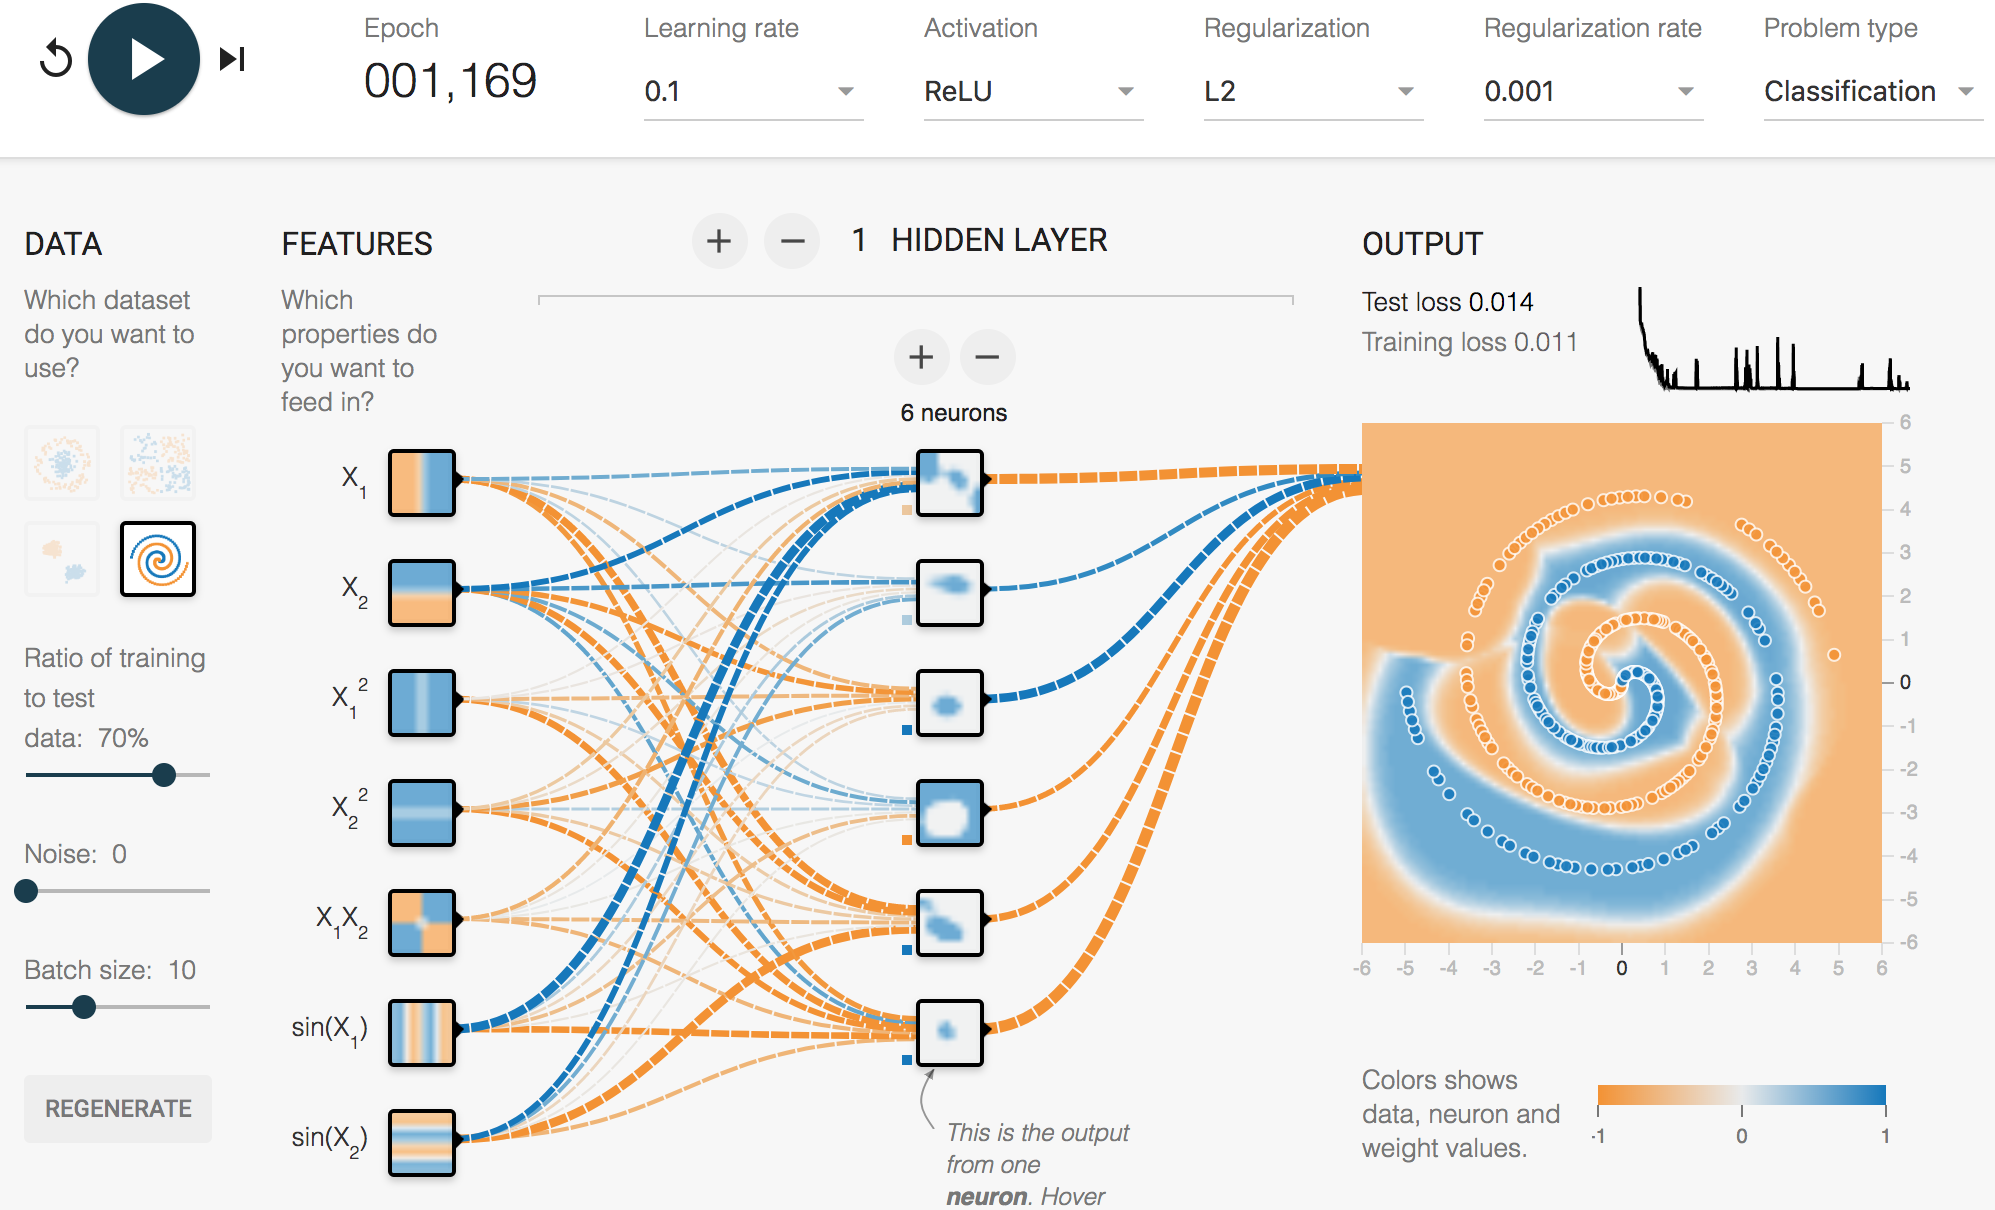
\includegraphics[scale=0.35]{1.png}
\caption{Use more features but fewer layers}
\label{fig:pathdemo}
\end{figure}
\par
As shown in figure 2, when only the two basic features but use more layers are used, the network can also achieve a good nonlinear performance.
\begin{figure}[ht]
\centering
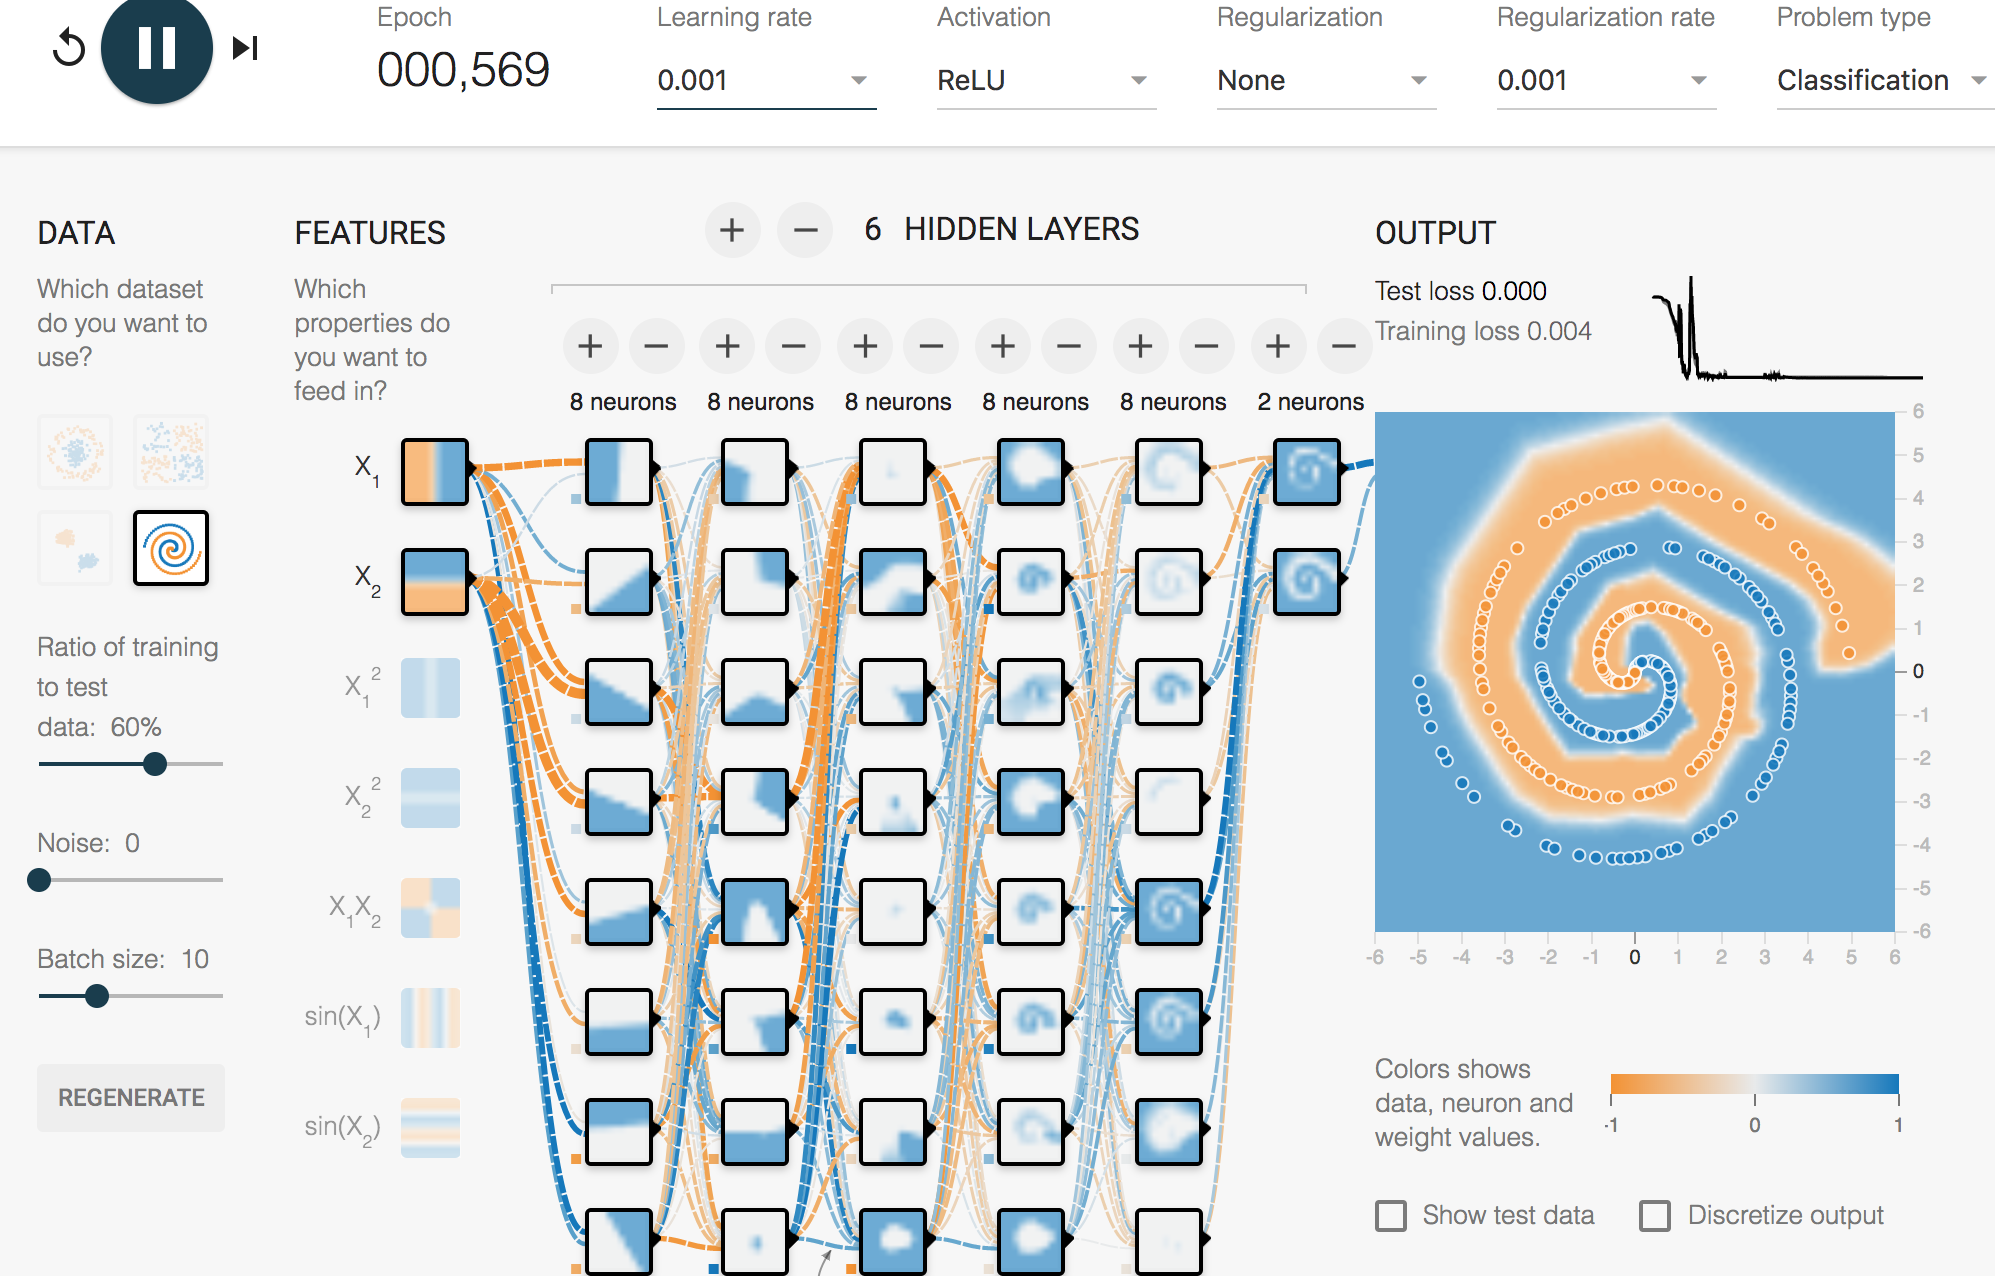
\includegraphics[scale=0.35]{2.png}
\caption{Use fewer features but more layers}
\end{figure}
\par
During the training, the learning rate is 0.1 for the first 400 epochs, 0.03 for the next 100 epochs, and 0.01 for the rest epochs. The batch size is set as 10 and the ratio of training to test is 60\%. The activation function is ReLU, and there is no regularization.
\par
\smallskip
2. In this dataset, regularization term is not a must. As shown in figure 2, test loss reaches 0 meaning that there is no overfitting, though there is no regularization.
\par
Also, in this dataset ReLU function can achieve a better performance compared with other activation functions such as Tanh, Sigmoid and Linear(I use all activation functions training the network for 500 epochs, the testing loss with ReLU function is the lowest). 
\par
At the beginning of the training, the learning rate is set as 0.1 in order to speed up the learning process. At the end of the training, the learning rate needs diminishing so that the loss will not oscillate. Also, during this training, setting the batch size to 10 seems a fairly good choice since it can avoid large variance, avoid local minimum, and the training time is also acceptable.
\par
\smallskip
3. During the training, there are several details need to be adjusted carefully:
\par
(1) Usually ReLU is the best choice for activation function.
\par
(2) Choosing a good learning rate is important, sometimes we can use an auto decaying learning rate, or just diminish the learning rate after some epochs. 
\par
(3) Batch normalization can accelerate training process. 
\par
(4) The initialization needs also adjusting, sometimes use uniform initialization and sometimes Xavier Initialization or He Initialization works better. 
\par 
(5) We can use regularization(such as L1, L2) or Dropout(default 0.5, sometimes 0.2 if the model is not very complicated) to avoid overfitting. 
\par 
(6) Choose a good optimizer method from various methods such as Adagrad, RMSProp.

\bigskip
{\large \bf 3 Clustering: Mixture of Multinomials}
\par
\bigskip
{\bf 3.1 MLE for multinomial}
\par
For multinomial distribution:
$$P(\bm{x}|\bm{\mu})=\frac{n!}{\prod_{i=1}^d x_i!}\prod_{i=1}^d \mu_i^{x_i},\,i=1,\cdots,d$$
where $x_i\in\mathbb{N},$ $\sum_{i=1}^d x_i=n$, and the parameter $\bm{\mu}=(\mu_i)_{i=1}^d$, $0<\mu_i<1,$ $\sum_{i=1}^d\mu_i=1$.
\par
The log likelihood for $P(\bm{x}|\bm{\mu})$:
\begin{align*}
\log P(\bm{x}|\bm{\mu})&=\log(n!)-\sum_{i=1}^d\log(x_i!)+\sum_{i=1}^d x_i\log(\mu_i)
\end{align*}
Maximize the log likelihood w.r.t. $\bm{\mu}$, and consider the constraint $\sum_{i=1}^d\mu_i=1$. Therefore, first derive the Lagrange function of $\log P(\bm{x}|\bm{\mu})$:
\begin{align*}
L(\bm{\mu},\beta)=\log(n!)-\sum_{i=1}^d\log(x_i!)+\sum_{i=1}^d x_i\log(\mu_i)-\beta\left(\sum_{i=1}^d\mu_i-1\right)
\end{align*}
where $\beta$ is Lagrange multipliers.
\par
Solve the gradient of $L(\bm{\mu},\beta)$ w.r.t. $\bm{\mu},\,\bm{\alpha}$ and the derivative w.r.t. $\beta$ are:
\begin{align*}
&\nabla_{\bm{\mu}}L(\bm{\mu},\beta)=\left[\frac{x_1}{\mu_1}-\beta,\frac{x_2}{\mu_2}-\beta,\cdots,\frac{x_d}{\mu_d}-\beta\right]^T\\
&\frac{\partial L(\bm{\mu},\beta)}{\beta}=-\sum_{i=1}^d\mu_i+1
\end{align*}
Let them equal to zero, there are $\mu_i=\frac{x_i}{\beta},\,i=1,2,\cdots,d$, and $\sum_{i=1}^d\mu_i=1$. Therefore:
$$\sum_{i=1}^d\mu_i=\sum_{i=1}^d\frac{x_i}{\beta}=1\Rightarrow\sum_{i=1}^d x_i=\beta=n$$
So the maximum-likelihood estimator for the parameter $\bm{\mu}$ is:
$$\mu_i=\frac{x_i}{n},\,i=1,2,\cdots,d$$
which also satisfies $0<\mu_i<1$.
\par
For $N$ samples, the gradient of $\tilde{L}(\bm{\mu},\beta)$ w.r.t. $\bm{\mu},\,\bm{\alpha}$ and the derivative w.r.t. $\beta$ are:
\begin{align*}
&\nabla_{\bm{\mu}}\tilde{L}(\bm{\mu},\beta)=\left[\sum_{n=1}^N\frac{x_{n1}}{\mu_1}-\beta,\sum_{n=1}^N\frac{x_{n2}}{\mu_2}-\beta,\cdots,\sum_{n=1}^N\frac{x_{nd}}{\mu_d}-\beta\right]^T\\
&\frac{\partial\tilde{L}(\bm{\mu},\beta)}{\beta}=-\sum_{i=1}^d\mu_i+1
\end{align*}
Therefore for $N$ samples, the maximum-likelihood estimator for $\bm{\mu}$ is:
$$\mu_i=\frac{\sum_{n=1}^N x_{ni}}{\sum_{j=1}^d\sum_{n=1}^N x_{nj}}=\frac{1}{Nn}\sum_{n=1}^N x_{ni},\,i=1,2,\cdots,d$$
which satisfies $0<\mu_i<1$.
\par
\bigskip
{\bf 3.2 EM for mixture of multinomials}
\par
The log likelihood of $D$ documents is:
\begin{align*}
J(\bm{\pi},\bm{\mu})&=\log\prod_{d=1}^D P(d)\\
&=\sum_{d=1}^D\log\sum_{k=1}^K P(d|c_d=k)P(c_d=k)\\
&=\sum_{d=1}^D\log\frac{n_d!}{\prod_{\omega=1}^WT_{d\omega}!}\sum_{k=1}^K\pi_k\prod_{\omega=1}^W\mu_{\omega k}^{T_{d\omega}}\\
&=\sum_{d=1}^D\log\frac{n_d!}{\prod_{\omega=1}^WT_{d\omega}!}+\sum_{d=1}^D\log\sum_{k=1}^K\pi_k\prod_{\omega=1}^W\mu_{\omega k}^{T_{d\omega}}\\
&=\sum_{d=1}^D\log\frac{n_d!}{\prod_{\omega=1}^WT_{d\omega}!}+\sum_{d=1}^D\log\sum_{k=1}^K q(z_d=k)\frac{\pi_k\prod_{\omega=1}^W\mu_{\omega k}^{T_{d\omega}}}{q(z_d=k)}\\
&\geq \sum_{d=1}^D\log\frac{n_d!}{\prod_{\omega=1}^WT_{d\omega}!}+\sum_{d=1}^D\sum_{k=1}^K q(z_d=k)\log\frac{\pi_k\prod_{\omega=1}^W\mu_{\omega k}^{T_{d\omega}}}{q(z_d=k)}
\end{align*}
where $q(z_d=k)=P(c_d=k|d)$ is the posterior distribution, and the inequality holds due to the Jensen inequality.
\par
Denote $\tilde{J}(q,\bm{\pi},\bm{\mu})$ as:
$$\tilde{J}(q,\bm{\pi},\bm{\mu})=\sum_{d=1}^D\sum_{k=1}^K q(z_d=k)\log\frac{\pi_k\prod_{\omega=1}^W\mu_{\omega k}^{T_{d\omega}}}{q(z_d=k)}$$
The {\bf E-step} is to update the posterior of the $(t+1)$th iteration $q^{(t+1)}(z_d=k),\,d=1,\cdots,D,\,k=1,\cdots,K$. 
\par 
Denote $q^{(t+1)}(z_d=k)$ as $\gamma_d^{(t+1)}(k)$, where $\sum_{k=1}^K\gamma_d^{(t+1)}(k)=1$. There is:
\begin{align*}
\gamma_d^{(t+1)}(k)=P(c_d=k|d)=\frac{P(c_d=k,d)}{\sum_{k=1}^K P(c_d=k,d)}=\frac{\pi_k^{(t)}\prod_{\omega=1}^W\mu_{\omega k}^{(t)T_{d\omega}}}{\sum_{k=1}^K\pi_k^{(t)}\prod_{\omega=1}^W\mu_{\omega k}^{(t)T_{d\omega}}}
\end{align*}
where $k=1,\cdots,K$.
\par
$\gamma_d^{(t+1)}(k)$ can be written as below in order to avoid overflow of $\mu_{\omega k}^{(t)T_{d\omega}}$:
\begin{align*}
\gamma_d^{(t+1)}(k)&=\exp\left[\log\gamma_d^{(t+1)}(k)\right]\\
&=\exp\left[\log\left(\pi_k^{(t)}\prod_{\omega=1}^W\mu_{\omega k}^{(t)T_{d\omega}}\right)-\log\sum_{k=1}^K\left(\pi_k^{(t)}\prod_{\omega=1}^W\mu_{\omega k}^{(t)T_{d\omega}}\right)\right]\\
&=\exp\left[a_k-\log\sum_{k=1}^K\exp\left(a_k\right)\right]\\
&=\exp\left[a_k-\log\sum_{k=1}^K\exp\left(a_k-max_a\right)\exp\left(max_a\right)\right]\\
&=\exp\left[a_k-max_a-\log\sum_{k=1}^K\exp\left(a_k-max_a\right)\right]
\end{align*}
where $a_k=\log\left(\pi_k^{(t)}\prod_{\omega=1}^W\mu_{\omega k}^{(t)T_{d\omega}}\right)=\log\pi_k^{(t)}+\sum_{\omega=1}^W T_{d\omega}\log\mu_{\omega k}^{(t)}$, $max_a=\max_{k}a$.

The {\bf M-step} is to update the parameters of the $(t+1)$th iteration $\bm{\pi}^{(t+1)},\bm{\mu}^{(t+1)}$:
\begin{align*}
&\bm{\pi}^{(t+1)}=\mathop{\arg\max}_{\bm{\pi}}\tilde{J}\left(q^{(t+1)},\bm{\pi},\bm{\mu}^{(t)}\right)\\
&\bm{\mu}^{(t+1)}=\mathop{\arg\max}_{\bm{\mu}}\tilde{J}\left(q^{(t+1)},\bm{\pi}^{(t+1)},\bm{\mu}\right)
\end{align*}
Considering the constraints $\sum_{k=1}^K\pi_k=1,\,\sum_{\omega=1}^W\mu_{\omega k}=1,\,k=1,\cdots,K$, use Lagrange functions $L(\bm{\pi},\bm{\mu})$ to solve the maximum problems. There are:
\begin{align*}
&\sum_{d=1}^D\frac{\gamma_d^{(t+1)}(k)}{\pi_k}-\beta=0,\,\sum_{k=1}^K\pi_k=1\;\Rightarrow\;
\pi_k^{(t+1)}=\frac{\sum_{d=1}^D\gamma_d^{(t+1)}(k)}{\sum_{k=1}^K\sum_{d=1}^D\gamma_d^{(t+1)}(k)}\\
&\sum_{d=1}^D\frac{\gamma_d^{(t+1)}(k)T_{d\omega}}{\mu_{\omega k}}-\beta=0,\,\sum_{\omega=1}^W\mu_{\omega k}=1\;\Rightarrow\;\mu_{\omega k}^{(t+1)}=\frac{\sum_{d=1}^D\gamma_d^{(t+1)}(k)T_{d\omega}}{\sum_{\omega=1}^W\sum_{d=1}^D\gamma_d^{(t+1)}(k)T_{d\omega}}
\end{align*}
where $k=1,\cdots,K$, $\omega=1,\cdots,W$.
\par
My program depends on Python packages {\bf numpy}, {\bf os}, {\bf tqdm} and {\bf sklearn}. There are two Python files: {\bf main.py} contains reading data, removing stopping words, EM procedure and results; {\bf evaluate.py} is to evaluate the results by using Adjusted Mutual Information. 
\par
The results are shown in {\bf outputs/}, containing topics and 5 most frequency words for $K=5,10,20,30$ respectively and the evaluation result. The evaluation result shows that the best $K$ value for this dataset is $20$, because the Adjusted Mutual Information score when $K=20$ is the highest among the scores when $K=5,10,20,30$ (AMI = 0.038, 0.050, 0.056, 0.055 respectively). 
\par
~\\
{\bf Most frequent words:}
\par
{\bf K=5:}
\begin{multicols}{2}
\par
For topic 0:
\par
'writes' 'people' 'article' 'don' 'time' \par
For topic 1:
\par
'people' 'god' 'don' 'writes' 'article' 
\par

For topic 2:
\par
'writes' 'article' 'don' 'people' 'good' \par
For topic 3:
\par
'writes' 'article' 'don' 'good' 'people' 
\par
For topic 4:
\par
'don' 'writes' 'key' 'people' 'article' 
~\\
~\\
\end{multicols}
\par
{\bf K=10:}
\par
\begin{multicols}{2}
For topic 0:
\par
'writes' 'article' 'people' 'time' 'don' \par
For topic 1:
\par
'writes' 'don' 'article' 'people' 'windows' \par
For topic 2:
\par
'writes' 'article' 'people' 'god' 'don' \par
For topic 3:
\par
'writes' 'article' 'scsi' 'don' 'people' \par
For topic 4:
\par
'god' 'writes' 'people' 'don' 'article' \par
For topic 5:
\par
'db' 'people' 'article' 'writes' 'space' \par
For topic 6:
\par
'don' 'people' 'writes' 'article' 'file' \par
For topic 7:
\par
'writes' 'article' 'don' 'apr' 'ca' \par
For topic 8:
\par
'writes' 'article' 'people' 'don' 'space' \par
For topic 9:
\par
'writes' 'people' 'don' 'article' 'good'
\end{multicols}
\par
{\bf K=20:}
\par
\begin{multicols}{2}
For topic 0:
\par
'writes' 'article' 'don' 'good' 'apr' \par
For topic 1:
\par
'writes' 'article' 'people' 'don' 'gun' \par
For topic 2:
\par
'people' 'window' 'don' 'writes' 'article' \par
For topic 3:
\par
'writes' 'article' 'people' 'time' 'good' \par
For topic 4:
\par
'writes' 'article' 'don' 'people' 'good' \par
For topic 5:
\par
'writes' 'article' 'space' 'don' 'data' \par
For topic 6:
\par
'writes' 'article' 'file' 'output' 'don' \par
For topic 7:
\par
'scsi' 'drive' 'mb' 'card' 'bit' \par
For topic 8:
\par
'god' 'mr' 'don' 'stephanopoulos' 'writes' \par
For topic 9:
\par
'db' 'writes' 'article' 'people' 'time' \par
For topic 10:
\par
'writes' 'article' 'don' 'time' 'people' \par
For topic 11:
\par
'people' 'writes' 'article' 'hockey' 'don' \par
For topic 12:
\par
'writes' 'key' 'encryption' 'article' 'chip' \par
For topic 13:
\par
'people' 'space' 'don' 'writes' 'time' \par
For topic 14:
\par
'writes' 'people' 'article' 'don' 'time' \par
For topic 15:
\par
'don' 'people' 'writes' 'jpeg' 'good' \par
For topic 16:
\par
'god' 'people' 'writes' 'article' 'don' \par
For topic 17:
\par
'people' 'writes' 'god' 'article' 'file' \par
For topic 18:
\par
'writes' 'jews' 'article' 'turkish' 'years' \par
For topic 19:
\par
'writes' 'article' 'don' 'good' 'people' 
\end{multicols}
\par 
{\bf K=30:}
\par
\begin{multicols}{2}
For topic 0:
\par
'writes' 'don' 'game' 'year' 'people' \par
For topic 1:
\par
'writes' 'information' 'don' 'time' 'people' \par
For topic 2:
\par
'god' 'people' 'writes' 'article' 'don' \par
For topic 3:
\par
'writes' 'article' 'don' 'people' 'ca' \par
For topic 4:
\par
'writes' 'article' 'time' 'don' 'people' \par
For topic 5:
\par
'db' 'mov' 'space' 'bh' 'cs' \par
For topic 6:
\par
'writes' 'article' 'don' 'good' 'time' \par
For topic 7:
\par
'people' 'god' 'writes' 'article' 'don' \par
For topic 8:
\par
'wire' 'ground' 'wiring' 'people' 'good' \par
~\\
~\\
For topic 9:
\par
'writes' 'article' 'ftp' 'people' 'don' \par
For topic 10:
\par
'writes' 'ms' 'myers' 'article' 'don' \par
For topic 11:
\par
'mr' 'stephanopoulos' 'don' 'people' 'writes' \par
For topic 12:
\par
'writes' 'people' 'article' 'don' 'time' \par
For topic 13:
\par
'file' 'output' 'don' 'people' 'program' \par
For topic 14:
\par
'writes' 'don' 'article' 'time' 'system' \par
For topic 15:
\par
'writes' 'article' 'people' 'apr' 'don' \par
For topic 16:
\par
'writes' 'article' 'turkish' 'people' 'don' \par
For topic 17:
\par
'don' 'writes' 'article' 'israel' 'people' \par
~\\
~\\
For topic 18:
\par
'writes' 'article' 'don' 'time' 'good' \par
For topic 19:
\par
'people' 'jesus' 'writes' 'key' 'time' \par
For topic 20:
\par
'drive' 'writes' 'don' 'mb' 'scsi' \par
For topic 21:
\par
'scsi' 'article' 'writes' 'dos' 'gm' \par
For topic 22:
\par
'writes' 'article' 'don' 'people' 'apr' \par
For topic 23:
\par
'writes' 'article' 'god' 'file' 'drive' \par
For topic 24:
\par
'writes' 'drive' 'article' 'windows' 'scsi' \par
For topic 25:
\par
'god' 'writes' 'article' 'people' 'don' \par
For topic 26:
\par
'people' 'don' 'writes' 'image' 'time' \par
For topic 27:
\par
'writes' 'card' 'article' 'drive' 'time' \par
For topic 28:
\par
'writes' 'people' 'don' 'article' 'apr' \par
For topic 29:
\par
'encryption' 'writes' 'don' 'key' 'article' 
\end{multicols}

\end{document}